% Copyright 2021 by FIZ-Karlsruhe
%
% This file is part of the ctan package zbmath-review-template
% and may be distributed and/or modified under the
% conditions of the GNU General Public License, version 3:
%
% https://www.gnu.org/licenses/gpl-3.0.en.html
%
% It contains the manual for zbmath-review-template.
%


\documentclass{zbMATH}
\usepackage{hyperref}

\hypersetup{colorlinks=true,allcolors=[rgb]{0,.289,.6}}


\begin{document}

\makefooter


\blue{\LARGE{\textbf{LaTeX-Template for zbMATH Open Reviews}}}

\vspace{4ex}

This package contains the class zbMATH, which is used for reviews on zbMATH Open.
With the class zbMATH you can see how your review will look like at zbMATH Open and you can test whether your LaTeX-code will compile properly on our system. 

Be aware that we add further information to your review, for example the list of references of the reviewed article, and there might be manual changes to your review. Thus, the published version of your review on zbMATH Open will look different than on this template. 

\section*{How to use the class zbMATH}

First, load the class zbMATH
\begin{verbatim}
    \documentclass{zbMATH}
\end{verbatim}

Then, use
\begin{verbatim}
    \title{<title of the reviewed article>}
    \author{<authors of the reviewed article>}
\end{verbatim}
to set the title and author information of the article under review. This can be set before or after \verb|\begin{document}|. The title and footer of your review are generated via
\begin{verbatim}
    \maketitle
    \makefooter
\end{verbatim}
After these two commands, add the text of your review. At the end, you can add your name (and your location) using
\begin{verbatim}
    \reviewer{<your name (location)>}
\end{verbatim}
Optionally, you can add MSC Classes and keywords
\begin{verbatim}
    \msc{<MSC Classes>}
    \keywords{<keywords>}
\end{verbatim}
where MSC classes are separated by space and keywords are separated by ';'.

Finally, compile your \texttt{.tex} file using XeLaTeX. An example is given in zb-example.tex.

\section*{LaTeX Format}

Please prepare your review in standard LaTeX. You might use functions and macros from the following packages:
\begin{itemize}[nosep]
    \item \href{https://www.ams.org/arc/resources/amslatex-about.html}{amsmath, amsfonts, amssymb}
    \item \href{https://ctan.org/pkg/stmaryrd}{stmaryrd}
    \item \href{https://ctan.org/pkg/mathrsfs}{mathrsfs}
    \item \href{https://ctan.org/pkg/tikz-cd}{tikz-cd}
    \item \href{https://ctan.org/pkg/mathtools}{mathtools}
    \item \href{https://ctan.org/pkg/gensymb}{gensymb}
    \item \href{https://ctan.org/pkg/textcomp}{textcomp}
\end{itemize}
Furthermore, you might use the macros defined in zbMATH.cls, that are:
\begin{itemize}[nosep]
    \item \verb|\Im| and \verb|\Re| for the imaginary and real part of a complex number, for example, \(\Re(x+iy)=x\) and \(\Im(x+iy)=y\).
    \item \verb|\Aut| for the automorphism group of a set, e.g., \(\Aut(X)\) for a set \(X\).
    \item \verb|\Hom| for the hom-Functor, e.g., \(\Hom(A,B)\) stands for the set of homomorphisms from a set \(A\) to a set \(B\).
    \item \verb|\ran| for the range or image of a vector space, e.g., \(\ker A = \left(\ran A^*\right)^\bot\).
    \item \verb|\1| for the indicator function of a set, e.g.
    \[\1_A = \begin{cases}1 &\text{if }x\in A\\
    0 &\text{if }x\notin A
    \end{cases}.\]
    \item \verb|\fint| for \(\fint\), e.g.,
    \[\fint_A u(y)\,d\mu(y)=\frac{1}
    {\mu(A)}\int_A u(y)\,d\mu(y)\]
    \item \verb|\Sha| for the Tate–Shafarevich group $\Sha(A/K)$ of an abelian variety \(A\) defined over a number field \(K\).
\end{itemize}
Please do not use any self-defined macros or packages not listed above. If you feel that there is a missing package that we should add, please let us know.

Our PDFs are compiled using XeLaTeX, which supports unicode characters in the source files.
Unicode allows the user to include accents and special characters coming from different Asian and European languages. For example, you may enter accented characters directly (e.g., \verb|Lévy| instead of \verb|L\'evy|). 
However, please avoid including unicode characters in mathematical mode. 
In particular, when you type Greek characters for variables please use \verb|\(\beta\)| or \verb|$\beta$| obtaining \(\beta\), instead of typing the unicode character directly.

Please do not include tables, large diagrams, drawings or formulas of minor importance. Use alternative fonts (bold, italics etc.) only if necessary, e.g., in formulas or for highlighting the authors of cited publications.

\section*{Mathematical Typesetting}

When writing equations or diagrams please avoid the automatic numbering environments and replace them with their * analogues. For example, use 

\verb|\begin{equation*} \end{equation*}|

instead of 

\verb|\begin{equation} \end{equation}|. 

The numbers on equations, definitions, diagrams, etc. should be set manually. You can do this by typing, for instance, \verb|\tag{1}| or \verb|\tag{*}|.

For example
\begin{verbatim}
\begin{equation*}
  \sum_{n=1}^\infty \frac{1}{n^2} = \frac{\pi^2}{6} \tag{1}\label{eq:1}
\end{equation*}
\end{verbatim}
gives
\begin{equation*}
    \sum_{n=1}^\infty \frac{1}{n^2}=\frac{\pi^2}{6} \tag{1}\label{eq:1}
\end{equation*}
An equation can be referenced via \verb|\ref{key}| if it is labeled by \verb|\label{key}|. The formula above can be referenced via \verb|\ref{eq:1}|:

Equation~\ref{eq:1} was proven by Leonhard Euler in his paper \textit{De summis serierum reciprocarum}.

For inline mathematical formula we prefer to use \verb|\(...\)| over \verb|$...$|. Similarly, we recommend to use \verb|\[...\]| instead of \verb|$$...$$|.

\subsection*{Matrices}

We give a short description how to type matrices with \texttt{amsmath}. For more details we refer to the documentation of \href{https://www.ams.org/arc/resources/amslatex-about.html}{amsmath} on ctan.

\texttt{amsmath} provides several environments for matrices using different brackets. For example the code 
\begin{verbatim}
\[
\begin{pmatrix} a & b \\ c & d \end{pmatrix}\quad
\begin{matrix} a & b \\ c & d \end{matrix}\quad 
\begin{bmatrix} a & b \\ c & d \end{bmatrix}\quad
\begin{Bmatrix} a & b \\ c & d \end{Bmatrix}\quad
\begin{vmatrix} a & b \\ c & d \end{vmatrix} \quad
\begin{Vmatrix} a & b \\ c & d \end{Vmatrix}
\]
\end{verbatim}

generates these four matrices
\[
\begin{pmatrix} a & b \\ c & d \end{pmatrix}\quad
\begin{matrix} a & b \\ c & d \end{matrix}\quad 
\begin{bmatrix} a & b \\ c & d \end{bmatrix}\quad
\begin{Bmatrix} a & b \\ c & d \end{Bmatrix}\quad
\begin{vmatrix} a & b \\ c & d \end{vmatrix} \quad
\begin{Vmatrix} a & b \\ c & d \end{Vmatrix}.
\]

If you want to use a matrix in inline math mode, then you might use \verb|\smallmatrix|, e.g. \(\left(\begin{smallmatrix} 1&2\\ 3&4 \end{smallmatrix}\right)\) is typed via
\begin{verbatim}
\(\left(\begin{smallmatrix} 1&2\\ 3&4 \end{smallmatrix}\right)\).
\end{verbatim}
Observe that you have to add your own deliminator to the smallmatrix environment, here we use \verb|\left(| and \verb|\right)|.

\subsection*{Commutative Diagrams}

The package \texttt{tikz-cd} is designed to draw commutative diagrams. They are constructed inside the environment \verb|\begin{tikzcd}...\end{tikzcd}|. Its usage is similar to the one of tables (\verb|&| for columns and \verb|\\| for rows). Arrows are drawn using the command \verb|\arrow[options]|. The direction of an arrow is specified by a string of characters \texttt{r}, \texttt{l}, \texttt{u}, \texttt{d} (right, left, up, down) and labels are added using quotes \texttt{"<label>"}. We give examples of some commutative diagrams that occur regularly.

A short exact sequence 
\(
\begin{tikzcd}
    0\arrow[r] & A \arrow[r, "f"] & B\arrow[r, "g"] & C\arrow[r] & 0
\end{tikzcd}
\)
can be easily typed using \texttt{tikz-cd} by
\begin{verbatim}
\begin{tikzcd}
    0\arrow[r] & A \arrow[r, "f"] & B\arrow[r, "g"] & C\arrow[r] & 0
\end{tikzcd}
\end{verbatim}
The option \texttt{column sep} specifies the space between two consecutive columns. If we set this option to small
\begin{verbatim}
\begin{tikzcd}[column sep=small]
    0\arrow[r] &A \arrow[r, "f"] &B\arrow[r, "g"] &C\arrow[r] &0,
\end{tikzcd}
\end{verbatim}
the arrows of the short exact sequence 
\(
\begin{tikzcd}[column sep=small]
    0\arrow[r] & A \arrow[r, "f"] & B\arrow[r, "g"] & C\arrow[r] & 0
\end{tikzcd}
\)
are shorter.

Next, we give an example of a classical "square" commutative diagram, where we use \verb|column sep| and \verb|row sep| to specify the space between consecutive columns and rows, respectively. The diagram
\[
\begin{tikzcd}[column sep=large, row sep=large]
    A \arrow[r, "f"] \arrow[d, "g"] & B \arrow[d, "h"]\\
    C \arrow[r, "k"]& D
\end{tikzcd}
\]
is generated by
\begin{verbatim}
\[
\begin{tikzcd}[column sep=large, row sep=large]
    A \arrow[r, "f"] \arrow[d, "g"] & B \arrow[d, "h"] \\
    C \arrow[r, "k"] & D
\end{tikzcd}
\].
\end{verbatim}

A "triangular" diagram as
\[
\begin{tikzcd}[row sep = large]
    A\arrow[d, "\pi" ']\arrow[r, "f"] & B \\
    A/\ker(f)\arrow[ru, dashrightarrow, "\tilde f" '] &
\end{tikzcd}
\]
can be drawn using
\begin{verbatim}
\[
\begin{tikzcd}[row sep = large]
    A\arrow[d, "\pi" ']\arrow[r, "f"] & B \\
    A/\ker(f)\arrow[ru, dashrightarrow, "\tilde f" '] &
\end{tikzcd}
\].
\end{verbatim}

For more details on the use of \href{https://ctan.org/pkg/tikz-cd}{tikz-cd} we refer to its documentation on ctan where examples of more complicated diagrams are given.

\section*{Citations}

Citations to related work are always appreciated. You only need to cite the related work inside your review and do not have to add a reference section at the end of your text.

Please try to be as specific and accurate as possible so that the citation can be identified unambiguously. You  may use the \href{https://zbmath.org/}{zbMATH Document Search} or the \href{https://zbmath.org/citationmatching/}{zbMATH Citation Matcher} to look up citations. The Cite Button for the respective zbMATH item gives the citation in the proper format for a zbMATH Open review, see Figure~\ref{fig:cite}.

Example 1: Book article (\href{https://zbmath.org/?q=an\%3A0970.90052}{Zbl 0970.90052}).

{[\textit{A. Schrijver}, Theory of linear and integer programming. Repr. Chichester: Wiley (1998; Zbl 0970.90052)]}

Example 2: Journal article (\href{https://zbmath.org/?q=an\%3A0239.05111}{Zbl 0239.05111}).

{[\textit{L. Lovász}, Discrete Math. 2, 253--267 (1972; Zbl 0239.05111)]}

If you want to cite an article, which does not have a zbl number, you can use the following format:

Example 3: Journal article without zbl umber.

{[\textit{Authors}, "Title", Journal Volume, Issue, pages (year)]}

\begin{figure}[bth]
    \centering
    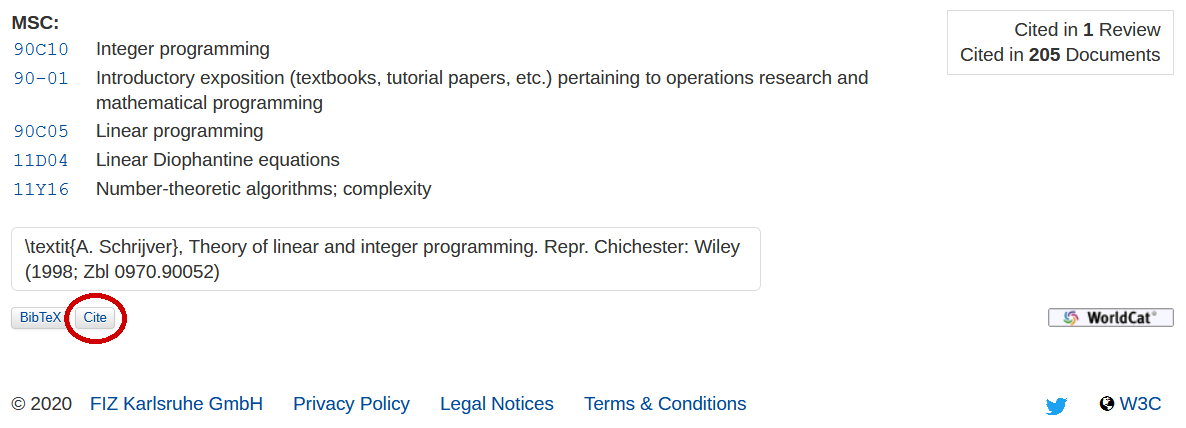
\includegraphics[width=\textwidth]{figures/screenshot.png}
    \caption{Cite Button at zbmath.org.}
    \label{fig:cite}
\end{figure}

If a Preprint should be cited, first check if there already exists a published version and cite the published article if it exists. Otherwise, cite the Preprint with as much information as possible, e.g. which University produced the Preprint, on which Preprint server did it appear together with a unique persistent identifier, if one exists. 

Example 4: A Preprint from arXiv

{[\textit{S. G. Hermosillo de la Maza} et al., “Vertex arboricity of cographs”, Preprint, \href{https://arxiv.org/abs/1907.07286}{arXiv:1907.07286}]}

\section*{Review Submission}

We prefer to receive your review electronically via our \href{https://zbmath.org/reviewer-service/}{Web Submission Form}. Just copy the text of your review into the field for the review text, please do not copy any of the macros \verb|\title|, \verb|\author|, \verb|\maketitle|, \verb|\makefooter|, \verb|\reviewer|, \verb|\msc|, \verb|\keywords|. There are two extra fields for keywords and MSC codes, respectively.

Alternatively, you may send your review by e-mail to review-submission@zbmath.org or via mail to our \href{https://zbmath.org/contact/}{postal address}.

For more information on the zbMATH Open Reviewer Service we refer to our \href{https://zbmath.org/reviewer-service/info_texts/guide_for_reviewers}{guide for reviewers}.

\section*{License}

The ctan package zbmath-review-template is distributed under the \href{https://www.gnu.org/licenses/gpl-3.0.en.html}{GNU General Public License, version 3}, except of zb-example.tex and zb-example.pdf, which are distributed under \href{https://creativecommons.org/licenses/by-sa/4.0/}{CC-BY-SA 4.0}.

\end{document}